\chapter{Parameter der Simulation}
\label{chap:ParameterDerSimulation}

\section{Maschinenparameter}\label{sec:maschinenparameter}

\subsection{Asynchronmaschine}\label{subsec:asynchronmaschine}


\begin{longtable}[]{@{}ll@{}}
\caption{Parameter für den Netzanschluss der
Asynchronmaschine}\tabularnewline
\toprule
Parameter & Wert\tabularnewline
\midrule
\endfirsthead
\toprule
Parameter & Wert\tabularnewline
\midrule
\endhead
\texttt{terminalBox1.terminalConnection} & ``D''\tabularnewline
\bottomrule
\end{longtable}

% -- Wicklungsdaten --
\begin{longtable}[]{@{}llll@{}}
\caption{Wicklungsdaten der Asynchronmaschine, entnommen aus \cite{pillerpowersystemsASMTIF2004}}\label{tab:WicklungsdatenASM}\tabularnewline
\toprule
Parameter              & Symbol                    & Wert          & Berechnung\tabularnewline
\midrule
\endfirsthead
\toprule
Parameter              & Symbol                    & Wert          & Berechnung\tabularnewline
\midrule
\endhead
Windungszahl           & $\hat N$                  & 56            & -\tabularnewline
Polpaarzahl            & $p$                       & 1             & -\tabularnewline
Nutzahl                & $Q$                       & 36            & -\tabularnewline
Stränge                & $m$                       & 3             & -\tabularnewline
Nutschritt             & $y_\mathrm{Q}$            & 10            & -\tabularnewline\midrule
Lochzahl               & $q$                       & 6             & $\frac{Q}{2pm}$\tabularnewline
Zonenfaktor            & $\xi_z$                   & 0,16666666667 & $\sin(\frac{\Delta\gamma _{\mathrm{c}}}{2})$\tabularnewline
Sehnungsfaktor         & $\xi_c$                   & 0,98260765    & $\frac{\sin(\frac{\pi}{6})}{q\sin(\frac{\pi}{6q})}$\tabularnewline
Nuten je Polpaar       & $S'$                      & 18            & $\frac{Q}{2p}$\tabularnewline
Spulenweite            & $\Delta\gamma_\mathrm{c}$ & 28,6478898    & $2\pi\cdot\frac{y_\mathrm{Q}}{S'}$\tabularnewline
effektive Windungszahl & $N_\mathrm{eff.s}$        & 9,17100475    & $\hat N\cdot\xi_\mathrm{c}\cdot\xi_\mathrm{z}$\tabularnewline
\bottomrule
\end{longtable}

% -- Daten aus Auslegung --
\begin{longtable}[]{@{}ll@{}}
\caption{Werte des Parameterrecords (\texttt{Fre­quenz­um­for­mer.­Ma­schi­nen­pa­ra­me­ter.­AIM\_­Squir­rel­Cage­Da­ta}) der Asynchronmaschine}\label{tab:WerteParameterrecordASM}\tabularnewline
\toprule
Parameter                     & Wert     \\
\midrule
\endfirsthead
\caption{Werte des Parameterrecords (\texttt{Fre­quenz­um­for­mer.­Ma­schi­nen­pa­ra­me­ter.­AIM\_­Squir­rel­Cage­Da­ta}) der Asynchronmaschine}\tabularnewline
\toprule
Parameter                     & Wert     \\
\midrule
\endhead
\texttt{Jr}                   & 0        \\
\texttt{L0}                   & 0        \\
\texttt{Rr}                   & 0,120    \\
\texttt{Rs}                   & 0,083574 \\
\texttt{X0}                   & 14,83    \\
\texttt{X1}                   & 0,448208 \\
\texttt{X2}                   & 0,791    \\
\texttt{effectiveStatorTurns} & 9,171    \\
\texttt{p}                    & 1        \\
\texttt{fsNominal}            & 50       \\
\bottomrule
\end{longtable}

% -- endgültige Parameter --
\begin{longtable}[]{@{}lll@{}}
\caption{Parameter des Modells der Asynchronmaschine (\texttt{Fun­da­men­tal­Wave.­Basic­Ma­chines.­Asyn­chro­nous­In­duc­tion­Ma­chines.­AIM\_­Squir­rel­Cage})}\label{tab:ParameterASM}\tabularnewline
\toprule
Parameter                     & Wert                                              & Berechnung\tabularnewline
\midrule
\endfirsthead
\toprule
Parameter                     & Wert                                              & Berechnung\tabularnewline
\midrule
\endhead
\texttt{Jr}                   & \texttt{aimcData.Jr}                              & \\
\texttt{Js}                   & \texttt{aimcData.Js}                              & \\
\texttt{phiMechanical}        & \texttt{(displayUnit="rad", fixed=false)}         & \\
\texttt{useSupport}           & \texttt{false}                                    & \\
\texttt{wMechanical}          & \texttt{(displayUnit = "rev/min", fixed = false)} & \\
\texttt{Lm}                   & \texttt{aimcData.Lm}                              & $\frac{X_0}{2\pi f_{s,Nominal}}$\\
\texttt{Lrsigma}              & \texttt{aimcData.Lrsigma}                         & $\frac{X_1}{2\pi f_{s,Nominal}}$\\
\texttt{Lssigma}              & \texttt{(fixed=false)}                            & $\frac{X_2}{2\pi f_{s,Nominal}}$\\
\texttt{Rr}                   & \texttt{aimcData.Rr}                              & \\
\texttt{Rs}                   & \texttt{(fixed=true,\ start=aimcData.Rs)}         & \\
\texttt{effectiveStatorTurns} & \texttt{aimcData.effectiveStatorTurns}            & \\
\texttt{fsNominal}            & \texttt{aimcData.fsNominal}                       & \\
\texttt{m}                    & \texttt{m}                                        & \\
\texttt{p}                    & \texttt{aimcData.p}                               & \\
\texttt{TrOperational}        & 293,15, \texttt{displayUnit = ''K''}              & \\
\texttt{TrRef}                & 293,15, \texttt{displayUnit = ''K''}              & \\
\texttt{TsOperational}        & 293,15, \texttt{displayUnit = ''K''}              & \\
\texttt{TsRef}                & 293,15, \texttt{displayUnit = ''K''}              & \\
\texttt{alpha20r}             & 0, \texttt{displayUnit = ''K''}                   & \\
\texttt{alpha20s}             & 0, \texttt{displayUnit = ''K''}                   & \\
\bottomrule
\end{longtable}

\begin{figure}[H]
	\centering
	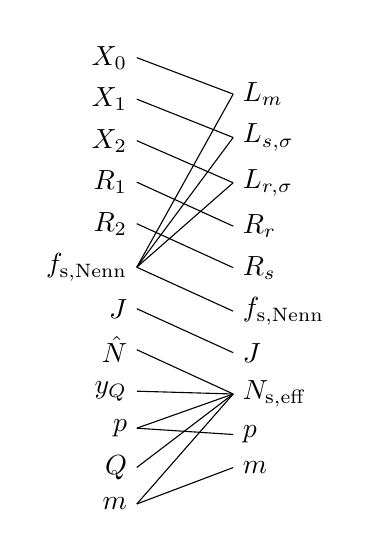
\begin{tikzpicture}[node distance=.5cm]
    % Linke Seite
    \begin{scope}[]
    	    \matrix[column 1/.style={anchor=base east}]{
             \node[] (X0) {$X_0$}; \\
             \node[] (X1) {$X_1$}; \\
             \node[] (X2) {$X_2$}; \\
             \node[] (R1) {$R_1$}; \\
             \node[] (R2) {$R_2$}; \\
             \node[] (fsNennl) {$f_{\mathrm{s,Nenn}}$};\\
             \node[] (Jl) {$J$};\\
             \node[] (N) {$\hat N$};\\
             \node[] (yQ) {$y_Q$};\\
             \node[] (pl) {$p$};\\
             \node[] (Q) {$Q$};\\
             \node[] (ml) {$m$};\\
        };
    \end{scope}
    % Rechte Seite
    \begin{scope}[xshift=2.5cm]
    	    \matrix[column 1/.style={anchor=base west}]{
             \node[] (Lm) {$L_m$}; \\
             \node[] (Lssigma) {$L_{s,\sigma}$};\\
             \node[] (Lrsigma) {$L_{r,\sigma}$};\\
             \node[] (Rr) {$R_r$};\\
             \node[] (Rs) {$R_s$};\\
             \node[] (fsNenn) {$f_{\mathrm{s,Nenn}}$};\\
             \node[] (J) {$J$};\\
             \node[] (Neff) {$N_{\mathrm{s,eff}}$};\\
             \node[] (p) {$p$};\\
             \node[] (m) {$m$};\\
        };
    \end{scope}
    \draw (Lm.west) edge (X0.east)
                    edge (fsNennl.east);

    \draw (Lssigma.west) edge (X1.east)
                    edge (fsNennl.east);

    \draw (Lrsigma.west) edge (X2.east)
                    edge (fsNennl.east);

    \draw (Neff.west) edge (N.east)
                      edge (pl.east)
                      edge (Q.east)
                      edge (ml.east)
                      edge (yQ.east);

    \draw (Rr.west) edge (R1.east);

    \draw (Rs.west) edge (R2.east);

    \draw (fsNenn.west) edge (fsNennl.east);

    \draw (p.west) edge (pl.east);

    \draw (m.west) edge (ml.east);

    \draw (J.west) edge (Jl.east);
\end{tikzpicture}

%             \node[] (XN) {$X_N$}; \\
%             \node[below=of XN] (XD) {$X_D$}; \\
%             \node[below=of XD] (XD') {$X_D'$}; \\
%             \node[below=of XD'] (XD'') {$X_D''$}; \\
%             \node[below=of XD''] (XQ) {$X_Q$}; \\
%             \node[below=of XQ] (XQ'') {$X_Q''$}; \\
%             \node[below=of XQ''] (XS) {$X_S$}; \\
%             \node[below=of XS] (fsN) {$f_{s,N}$}; \\
%             \node[below=of fsN] (Rs) {$R_s$}; \\
%             \node[below=of Rs] (TD0') {$T_{D0}'$}; \\
%             \node[below=of TD0'] (TD'') {$T_D''$}; \\
%             \node[below=of TD''] (TQ'') {$T_Q''$}; \\
	\caption{Zusammenhang zwischen den Parametern aus der Auslegung und der Simulation der Asynchronmaschine \label{fig:WebASM}}
\end{figure}

\subsection{Synchrongenerator}\label{synchron-generator}

\begin{longtable}[]{@{}ll@{}}
\caption{Parameter für den Netzanschluss des Synchrongenerators} \label{tab:NetzSG}
\tabularnewline
\toprule
Parameter & Wert\tabularnewline
\midrule
\endfirsthead
\toprule
Parameter & Wert\tabularnewline
\midrule
\endhead
\texttt{terminalBox.terminalConnection} & ``Y''\tabularnewline
\bottomrule
\end{longtable}

\begin{longtable}[]{@{}ll@{}}
\caption{Parameter aus der Auslegung des Synchrongenerators, entnommen aus \cite{pillerpowersystemsTechnischeDatenSynchrongenerator,pillerpowersystemsWickelblattSynchrongenerator272004}} \label{tab:AuslegungSG}
\tabularnewline
\toprule
Parameter & Wert\tabularnewline
\midrule
\endfirsthead
\caption{Parameter aus der Auslegung des Synchrongenerators, entnommen aus \cite{pillerpowersystemsTechnischeDatenSynchrongenerator,pillerpowersystemsWickelblattSynchrongenerator272004}}\tabularnewline
\toprule
Parameter & Wert\tabularnewline
\midrule
\endhead
\(X_N\)     & \(\unit[0,44444444444444436]{\Omega}\)\tabularnewline
\(X_D\)     & \(\unit[0,37232409867781685]{\Omega}\)\tabularnewline
\(X_D'\)    & \(\unit[0,10727388372365276]{\Omega}\)\tabularnewline
\(X_D''\)   & \(\unit[0,063131689804932889]{\Omega}\)\tabularnewline
\(X_Q\)     & \(\unit[0,16268065808519006]{\Omega}\)\tabularnewline
\(X_Q''\)   & \(\unit[0,061911567284431417]{\Omega}\)\tabularnewline
\(X_0\)     & \(\unit[0,13773696682464454]{\Omega}\)\tabularnewline
\(X_S\)     & \(\unit[0,042106445136139446]{\Omega}\)\tabularnewline
\(f_{s,N}\) & \(\unit[400]{Hz}\)\tabularnewline
\(R_s\)     & \(\unit[6,68\cdot 10^{-3}]{\Omega}\)\tabularnewline
\(T_{D0}'\) & \(\unit[0,1075492579055312]{s}\)\tabularnewline
\(T_D''\)   & \(\unit[0,0038358105876696909]{s}\)\tabularnewline
\(T_Q''\)   & \(\unit[0,0028791616002136365]{s}\)\tabularnewline
$\hat N$    & 18 \tabularnewline
$\xi_\mathrm{c}\xi_\mathrm{z}$ & 0,831 \tabularnewline
\bottomrule
\end{longtable}

\begin{longtable}[]{@{}lll@{}}
\caption{Zwischenwerte und Berechnungsgleichungen für Parameter des Sychrongenerators}\label{tab:ZwischenwerteSG}
\tabularnewline
\toprule
Parameter & Wert & Berechnung\tabularnewline
\midrule
\endfirsthead
\toprule
Parameter & Wert & Berechnung\tabularnewline
\midrule
\endhead
\(\omega_{s,N}\) & \(\unit[2513,27412]{\frac{rad}{s}}\) & \(2\pi f_{s,N}\) \tabularnewline
\(x_d\).         & 0,83772922                           & \(\frac{X_D}{X_N}\) \tabularnewline
\(x_d'\)         & 0,24136624                           & \(\frac{X_D'}{X_N}\) \tabularnewline
\(x_d''\)        & 0,1420463                            & \(\frac{X_D''}{X_N}\) \tabularnewline
\(x_q\)          &  0,36603148                          & \(\frac{X_Q}{X_N}\) \tabularnewline
\(x_q''\)        & 0,13930103                           & \(\frac{X_Q''}{X_N}\) \tabularnewline
\(x_s\)          & 0,0947395                            & \(\frac{X_S}{X_N}\) \tabularnewline
\(x_{md}\)       & 0,74298972                           & \(x_d-x_s\) \tabularnewline
\(x_{mq}\)       & 0,27129198                           & \(x_q-x_s\)\tabularnewline
\(x_e\)          & 0,92566732                           & \(\frac{x_{md}^2}{x_d-x_d''}\)\tabularnewline
\(x_{rd}\)       & 0,81282909                           & \(\frac{x_{md}^2}{x_d'-x_d''}(1-\frac{x_{md}}{x_e})^2+\frac{x_{md}^2}{x_e}\) \tabularnewline
\(x_{rq}\)       & 0,32461161                           & \(\frac{x_{mq}^2}{x_q-x_q''}\) \tabularnewline
\(r_s\)          & 0,0150285                            & \(\frac{R_s}{X_N}\) \tabularnewline
\(r_{rd}\)       & 0,01321437                           & \(\frac{x_{rd}-\frac{x_{md}^2}{x_e}}{\omega_{s,N}T_{D0}''}\) \tabularnewline
\(r_{rq}\)       & 0,01707238                           & \(\frac{x_{rq}}{\omega_{s,N}T_{Q0}''}\) \tabularnewline
\(r_e\)          & 0,00342458                           & \(\frac{x_e}{\omega_{s,N}T_{D0'}}\) \tabularnewline
\(T_{d0}''\)     & \unit[0,00651784]{s}                 & \(\frac{x_d'}{x_d''}T_D''\) \tabularnewline
\(T_{Q0}''\)     & \unit[0,00756537]{s}                 & \(\frac{x_q}{x_q''}T_Q\) \tabularnewline
turnsratio       & 47,9934193                           & \(\frac{V_{\mathrm{s,Nominal}}}{\omega_{\mathrm{s,N}}L_{\mathrm{md}}I_{\mathrm{e,OpenCircuit}}}\) \tabularnewline
$N_\mathrm{eff,s}$& 14,958                              & $\hat N\cdot\xi_\mathrm{c}\xi_\mathrm{z}$ \tabularnewline
$\sigma_\mathrm{e}$& 0,1973 & $\frac{1-x_{\mathrm{md}}}{x_\mathrm e}$\tabularnewline
\bottomrule
\end{longtable}

\begin{longtable}[]{@{}lll@{}}
\caption{Werte des Parameterrecords (\texttt{Machines.­Utilities.­Parameter­Records.­SM\_­ElectricalExcited­Data}) für den Synchrongenerator}\label{tab:ParameterRecordSG}
\tabularnewline
\toprule
Parameter & Wert & Berechnung\\
\midrule
\endfirsthead
\toprule
Parameter & Wert & Berechnung\\
\midrule
\endhead
\texttt{Jr}                   & 0                  & \\
\texttt{IeOpenCircuit}        & 7,2563105523832900 & \\
\texttt{Lmd}                  & 131,389E-6         & $x_{\mathrm{md}}\cdot \frac{X_{\mathrm{N}}}{\omega_{\mathrm{sN}}}$\\
\texttt{Lmq}                  & 47,975E-6          & $x_{\mathrm{mq}}\cdot \frac{X_{\mathrm{N}}}{\omega_{\mathrm{sN}}}$\\
\texttt{Lrsigmad}             & 12,35031219E-6     & $(x_{\mathrm{rq}} - x_{\mathrm{mq}})\cdot \frac{X_{\mathrm{N}}}{\omega_{\mathrm{sN}}}$\\
\texttt{Lrsigmaq}             & 9,428981013E-6     & $(x_{\mathrm{rd}} - x_{\mathrm{md}})\cdot \frac{X_{\mathrm{N}}}{\omega_{\mathrm{sN}}}$\\
\texttt{Lssigma}              & 16,7536222E-6      & $x_{\mathrm{s}}\cdot \frac{X_{\mathrm{N}}}{\omega_{\mathrm{sN}}}$\\
\texttt{Re}                   & 6,8                & $\frac{3}{2}\cdot \left(\frac{\sqrt{2}U_{\mathrm{sNenn}}}{\omega_{\mathrm{sN}}L_{\mathrm{md}}\cdot I_{\mathrm{Err,Leerl.}}}\right)^2\cdot r_{\mathrm{e}}\cdot X_{\mathrm{N}}$\\
\texttt{Rrd}                  & 5,873051175E-3     & $r_{\mathrm{rd}}\cdot X_{\mathrm{N}}$\\
\texttt{Rrq}                  & 7,587723698E-3     & $r_{\mathrm{rq}}\cdot X_{\mathrm{N}}$\\
\texttt{Rs}                   & 0.006679333        & $r_{\mathrm{s}}\cdot X_{\mathrm{N}}$\\
\texttt{VsNominal}            & 115                & \\
\texttt{effectiveStatorTurns} & 14,958             & \\
\texttt{fsNominal}            & 400                & \\
\texttt{p}                    & 8                  & \\
\texttt{sigmae}               & 0,1973             & \\
\texttt{useDamperCage}        & \texttt{true}      & \\
\bottomrule
\end{longtable}

\begin{longtable}[]{@{}ll@{}}
\caption{Parameter des Modells des Synchrongenerators}\label{tab:ParameterSG}
\tabularnewline
\toprule
Parameter & Wert\tabularnewline
\midrule
\endfirsthead
\caption{Parameter des Modells des Synchrongenerators}\tabularnewline
\toprule
Parameter & Wert\tabularnewline
\midrule
\endhead
\texttt{Jr} & \texttt{smeeData.Jr}\tabularnewline
\texttt{Js} & \texttt{smeeData.Js}\tabularnewline
\texttt{phiMechanical} &
\texttt{(displayUnit="rad",\ fixed=false)}\tabularnewline
\texttt{useSupport} & \texttt{false}\tabularnewline
\texttt{wMechanical} &
\texttt{(displayunit="rev/min",\ fixed=false)}\tabularnewline
\texttt{IeOpenCircuit} & \texttt{smeeData.IeOpenCircuit}\tabularnewline
\texttt{Lmd} & \texttt{smeeData.Lmd}\tabularnewline
\texttt{Lmq} & \texttt{smeeData.Lmq}\tabularnewline
\texttt{Lrsigmad} & \texttt{smeeData.Lrsigmad}\tabularnewline
\texttt{Lrsigmaq} & \texttt{smeeData.Lrsigmaq}\tabularnewline
\texttt{Lssigma} &
\texttt{(fixed=false,\ start=smeeData.Lssigma)}\tabularnewline
\texttt{Re} & \texttt{smeeData.Re}\tabularnewline
\texttt{Rrd} & \texttt{smeeData.Rrd}\tabularnewline
\texttt{Rrq} & \texttt{smeeData.Rrq}\tabularnewline
\texttt{Rs} & \texttt{(fixed=false)}\tabularnewline
\texttt{VsNominal} & \texttt{smeeData.VsNominal}\tabularnewline
\texttt{effectiveStatorTurns} &
\texttt{smeeData.effectiveStatorTurns}\tabularnewline
\texttt{fsNominal} & \texttt{smeeData.fsNominal}\tabularnewline
\texttt{m} & \texttt{m}\tabularnewline
\texttt{p} & \texttt{smeeData.p}\tabularnewline
\texttt{TeOperational} &
\texttt{293,15\ (displayunit="K")}\tabularnewline
\texttt{TeRef} & \texttt{293,15\ (displayunit="K")}\tabularnewline
\texttt{TrOperational} &
\texttt{293,15\ (displayunit="K")}\tabularnewline
\texttt{TrRef} & \texttt{293,15\ (displayunit="K")}\tabularnewline
\texttt{TsOperational} &
\texttt{293,15\ (displayunit="K")}\tabularnewline
\texttt{TsRef} & \texttt{293,15\ (displayunit="K")}\tabularnewline
\texttt{alpha20e} & 0\tabularnewline
\texttt{alpha20r} & 0\tabularnewline
\texttt{alpha20s} & 0\tabularnewline
\bottomrule
\end{longtable}

\begin{figure}[H]
	\centering
	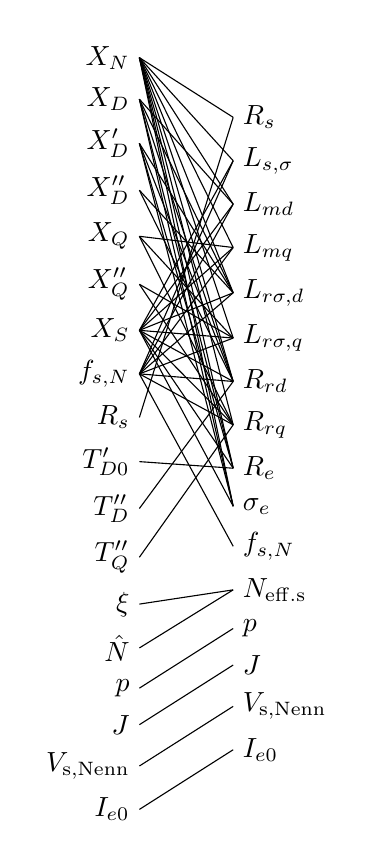
\begin{tikzpicture}[node distance=.5cm]
    % Linke Seite
    \begin{scope}[]
    	    \matrix[column 1/.style={anchor=base east}]{
             \node[] (XN) {$X_N$}; \\
             \node[] (XD) {$X_D$}; \\
             \node[] (XD') {$X_D'$}; \\
             \node[] (XD'') {$X_D''$}; \\
             \node[] (XQ) {$X_Q$}; \\
             \node[] (XQ'') {$X_Q''$}; \\
             \node[] (XS) {$X_S$}; \\
             \node[] (fsNl) {$f_{s,N}$}; \\
             \node[] (Rsl) {$R_s$}; \\
             \node[] (TD0') {$T_{D0}'$}; \\
             \node[] (TD'') {$T_D''$}; \\
             \node[] (TQ'') {$T_Q''$}; \\
             \node[] (xi) {$\xi$};\\
             \node[] (N) {$\hat N$};\\
             \node[] (pl) {$p$};\\
             \node[] (Jl) {$J$};\\             
             \node[] (VsNennl) {$V_{\mathrm{s,Nenn}}$};\\
             \node[] (Ie0l) {$I_{e0}$};\\
        };
    \end{scope}
    % Rechte Seite
    \begin{scope}[xshift=2.5cm]
    	    \matrix[column 1/.style={anchor=base west}]{
             \node[] (Rs) {$R_s$}; \\
             \node[] (Lssigma) {$L_{s,\sigma}$}; \\
             \node[] (Lmd) {$L_{md}$}; \\
             \node[] (Lmq) {$L_{mq}$}; \\
             \node[] (Lrsigmad) {$L_{r\sigma,d}$}; \\
             \node[] (Lrsigmaq) {$L_{r\sigma,q}$}; \\
             \node[] (Rrd) {$R_{rd}$}; \\
             \node[] (Rrq) {$R_{rq}$}; \\
             \node[] (Re) {$R_e$}; \\
             \node[] (sigmae) {$\sigma_e$};\\
             \node[] (fsN) {$f_{s,N}$}; \\
             \node[] (Neff) {$N_{\mathrm{eff.s}}$};\\
             \node[] (p) {$p$};\\
             \node[] (J) {$J$};\\
             \node[] (VsNenn) {$V_{\mathrm{s,Nenn}}$};\\
             \node[] (Ie0) {$I_{e0}$};\\
        };
    \end{scope}
    \draw (XN.east) edge (Rs.west)
               edge (Lssigma.west)
               edge (Lmd.west)
               edge (Lmq.west)
               edge (Lrsigmad.west)
               edge (Lrsigmaq.west)
               edge (Rrd.west)
               edge (Rrq.west)
               edge (Re.west)
               edge (sigmae.west);

    \draw (XD.east) edge (Lmd.west)
               edge (Lrsigmad.west)
               edge (Rrd.west)
               edge (Re.west)
               edge (sigmae.west);
               
    \draw (XD'.east) edge (Lrsigmad.west)
                edge (Rrd.west)
                edge (Re.west)
               edge (sigmae.west);
                
    \draw (XD''.east) edge (Lrsigmad.west)
                 edge (Rrd.west);
                 
    \draw (XQ.east) edge (Lmq.west)
               edge (Lrsigmaq.west)
               edge (Rrq.west);
               
    \draw (XQ''.east) edge (Lrsigmaq.west)
                 edge (Rrq.west);
                 
    \draw (XS.east) edge (Lssigma.west)
               edge (Lmd.west)
               edge (Lmq.west)
               edge (Lrsigmad.west)
               edge (Lrsigmaq.west)
               edge (Rrd.west)
               edge (Rrq.west)
               edge (Re.west)
               edge (sigmae.west);
               
    \draw (fsNl.east) edge (Lssigma.west)
                edge (Lmd.west)
                edge (Lmq.west)
                edge (Lrsigmad.west)
                edge (Lrsigmaq.west)
                edge (Rrd.west)
                edge (Rrq.west)
                edge (fsN.west);
                
    \draw (Rsl.east) edge (Rs.west);
    
    \draw (TD0'.east) edge (Re.west);
    
    \draw (TD''.east) edge (Rrd.west);
    
    \draw (TQ''.east) edge (Rrq.west);
    
    \draw (xi.east) edge (Neff.west);
    
    \draw (N.east) edge (Neff.west);

    \draw (pl.east) edge (p.west);
    
    \draw (Jl.east) edge (J.west);
    
    \draw (VsNennl.east) edge (VsNenn.west);
    
    \draw (Ie0l.east) edge (Ie0.west);    
\end{tikzpicture}

%             \node[] (XN) {$X_N$}; \\
%             \node[below=of XN] (XD) {$X_D$}; \\
%             \node[below=of XD] (XD') {$X_D'$}; \\
%             \node[below=of XD'] (XD'') {$X_D''$}; \\
%             \node[below=of XD''] (XQ) {$X_Q$}; \\
%             \node[below=of XQ] (XQ'') {$X_Q''$}; \\
%             \node[below=of XQ''] (XS) {$X_S$}; \\
%             \node[below=of XS] (fsN) {$f_{s,N}$}; \\
%             \node[below=of fsN] (Rs) {$R_s$}; \\
%             \node[below=of Rs] (TD0') {$T_{D0}'$}; \\
%             \node[below=of TD0'] (TD'') {$T_D''$}; \\
%             \node[below=of TD''] (TQ'') {$T_Q''$}; \\
	\caption{Zusammenhang zwischen den Parametern aus der Auslegung und der Simulation des Synchrongenerators \label{fig:WebSG}}
\end{figure}

\subsection{Erregermaschine}\label{sec:Erregermaschine}

\begin{longtable}[]{@{}ll@{}}
\caption{Parameter aus der Auslegung der Erregermaschine, entnommen aus \cite{pillerpowersystemsTechnischeDatenErregermaschine,pillerpowersystemsWickelblattErregermaschine272013}}\label{tab:AuslegungErregermaschine}
\tabularnewline
\toprule
Parameter & Wert\tabularnewline
\midrule
\endfirsthead
\toprule
Parameter & Wert\tabularnewline
\midrule
\endhead
\(X_N\)                            & \(\unit[3,249]{\Omega}\)    \\
\(X_D\)                            & \(\unit[28,75372]{\Omega}\) \\
\(X_D'\)                           & \(\unit[4,551998]{\Omega}\) \\
\(X_Q\)                            & \(\unit[12,73185]{\Omega}\) \\
\(X_S\)                            & \(\unit[2,438214]{\Omega}\) \\
\(f_{s,N}\)                        & \(\unit[148,5]{Hz}\)        \\
\(R_s\)                            & \(\unit[0,2205]{\Omega}\)   \\
\(T_{D0}'\)                        & \(\unit[0,04588457]{s}\)    \\
$N$                                & $108$ \\
$\xi_{\mathrm{c}}\xi_{\mathrm{z}}$ & $0,866$ \\
\bottomrule
\end{longtable}

\begin{longtable}[]{@{}lll@{}}
\caption{Zwischenwerte und Berechnungsgleichungen für Parameter der Erregermaschine}\label{tab:ZwischenwerteErregermaschine}
\tabularnewline
\toprule
Parameter & Wert & Berechnung \tabularnewline
\midrule
\endfirsthead
\caption{Zwischenwerte und Berechnungsgleichungen für Parameter der Erregermaschine}\tabularnewline
\toprule
Parameter & Wert & Berechnung \tabularnewline\midrule
\endhead
\(\omega_{s,N}\) & \(\unit[933,053018]{\frac{rad}{s}}\) & \(2\pi f_{s,N}\) \tabularnewline
\(x_d\) & 8,85002155 & \(\frac{X_D}{X_N}\) \tabularnewline
\(x_d'\) & 1,40104586 & \(\frac{X_D'}{X_N}\) \tabularnewline
\(x_q\) & 3,91869806 & \(\frac{X_Q}{X_N}\) \tabularnewline
\(x_s\) & 0,7504506 & \(\frac{X_S}{X_N}\) \tabularnewline
\(x_{md}\) & 8,09957094 & \(x_d-x_s\) \tabularnewline
\(x_{mq}\) & 3,16824746 & \(x_q-x_s\)\tabularnewline
\(x_e\) & 8,80698935 & \(\frac{x_{md}^2}{x_d-x_d''}\) \tabularnewline
\(r_s\) & 0,06786704 & \(\frac{R_s}{X_N}\) \tabularnewline
\(r_e\) & 0,20570956 & \(\frac{x_e}{\omega_{s,N}T_{D0'}}\) \tabularnewline
turnsratio & 1,49330662 & \(\frac{V_{\mathrm{s,Nominal}}}{\omega_{\mathrm{s,N}}L_{\mathrm{md}}I_{\mathrm{e,OpenCircuit}}}\)\tabularnewline
$\sigma_\mathrm{e}$& 0,0803 & $\frac{1-x_{\mathrm{md}}}{x_\mathrm e}$ \\
\bottomrule
\end{longtable}

\begin{longtable}[]{@{}lll@{}}
\caption{Werte des Parameterrecords (\texttt{Machines.­Utilities.­Parameter­Records.­SM\_­ElectricalExcited­Data}) für den Synchrongenerator der Erregermaschine}\label{tab:ParameterRecordErregermaschine}
\tabularnewline
\toprule
Parameter & Wert & Berechnung \\
\midrule
\endfirsthead
\toprule
Parameter & Wert & Berechnung \\
\midrule
\endhead
\texttt{Jr}                   & 0              & \\
\texttt{IeOpenCircuit}        & 1,450488       & \\
\texttt{Lmd}                  & 0,028203656    & $x_{\mathrm{md}}\cdot \frac{X_{\mathrm{N}}}{\omega_{\mathrm{sN}}}$\\
\texttt{Lmq}                  & 0,011032209    & $x_{\mathrm{mq}}\cdot \frac{X_{\mathrm{N}}}{\omega_{\mathrm{sN}}}$\\
\texttt{Lrsigmad}             & 0              & \\
\texttt{Lrsigmaq}             & 0              & \\
\texttt{Lssigma}              & 0,002613157    & $x_{\mathrm{s}}\cdot \frac{X_{\mathrm{N}}}{\omega_{\mathrm{sN}}}$\\
\texttt{Re}                   & 4,8            & $\frac{3}{2}\cdot \left(\frac{\sqrt{2}U_{\mathrm{sNenn}}}{\omega_{\mathrm{sN}}L_{\mathrm{md}}\cdot I_{\mathrm{Err,Leerl.}}}\right)^2\cdot r_{\mathrm{e}}\cdot X_{\mathrm{N}}$\\
\texttt{Rrd}                  & 0              & \\
\texttt{Rrq}                  & 0              & \\
\texttt{Rs}                   & 0.2205         & $r_{\mathrm{s}}\cdot X_{\mathrm{N}}$\\
\texttt{VsNominal}            & 57             & \\
\texttt{effectiveStatorTurns} & 93,528         & \\
\texttt{fsNominal}            & 148,5          & \\
\texttt{p}                    & 3              & \\
\texttt{sigmae}               & 0,0803         & \\
\texttt{useDamperCage}        & \texttt{false} & \\
\texttt{TeRef}                & 293,15         & \\
\texttt{TrRef}                & 293,15         & \\
\texttt{TsRef}                & 293,15         & \\
\texttt{alpha20e}             & 0              & \\
\texttt{alpha20r}             & 0              & \\
\texttt{alpha20s}             & 0              & \\
\bottomrule
\end{longtable}

\begin{longtable}[]{@{}ll@{}}
\caption{Parameter des Synchrongenerators der Erregermaschine} \label{tab:ParameterErregermaschine}
\tabularnewline
\toprule
Parameter & Wert\tabularnewline
\midrule
\endfirsthead
\toprule
Parameter & Wert\tabularnewline
\midrule
\endhead
\texttt{Jr} & \texttt{exciterData.Jr}\tabularnewline
\texttt{Js} & \texttt{exciterData.Js}\tabularnewline
\texttt{phiMechanical} & \texttt{(displayUnit="deg")}\tabularnewline
\texttt{useSupport} & \texttt{false}\tabularnewline
\texttt{wMechanical} & \texttt{(displayunit="rad/s")}\tabularnewline
\texttt{IeOpenCircuit} &
\texttt{exciterData.IeOpenCircuit}\tabularnewline
\texttt{Lmd} & \texttt{exciterData.Lmd}\tabularnewline
\texttt{Lmq} & \texttt{exciterData.Lmq}\tabularnewline
\texttt{Lrsigmad} & \texttt{exciterData.Lrsigmad}\tabularnewline
\texttt{Lrsigmaq} & \texttt{exciterData.Lrsigmaq}\tabularnewline
\texttt{Lssigma} &
\texttt{(fixed=false,\ start=smeeData.Lssigma)}\tabularnewline
\texttt{Re} & \texttt{exciterData.Re}\tabularnewline
\texttt{Rrd} & \texttt{exciterData.Rrd}\tabularnewline
\texttt{Rrq} & \texttt{exciterData.Rrq}\tabularnewline
\texttt{Rs} &
\texttt{(fixed=true,\ start=exciterData.Rs)}\tabularnewline
\texttt{VsNominal} & \texttt{exciterData.VsNominal}\tabularnewline
\texttt{effectiveStatorTurns} &
\texttt{exciterData.effectiveStatorTurns}\tabularnewline
\texttt{fsNominal} & \texttt{exciterData.fsNominal}\tabularnewline
\texttt{m} & 3\tabularnewline
\texttt{p} & \texttt{exciterData.p}\tabularnewline
\texttt{sigmae} & \texttt{exciterData.sigmae}\tabularnewline
\texttt{useDamperCage} & \texttt{false}\tabularnewline
\texttt{TeOperational} &
\texttt{293,15\ (displayunit="K")}\tabularnewline
\texttt{TeRef} & \texttt{293,15\ (displayunit="K")}\tabularnewline
\texttt{TrOperational} &
\texttt{293,15\ (displayunit="K")}\tabularnewline
\texttt{TrRef} & \texttt{293,15\ (displayunit="K")}\tabularnewline
\texttt{TsOperational} &
\texttt{293,15\ (displayunit="K")}\tabularnewline
\texttt{TsRef} & \texttt{293,15\ (displayunit="K")}\tabularnewline
\texttt{alpha20e} & 0\tabularnewline
\texttt{alpha20r} & 0\tabularnewline
\texttt{alpha20s} & 0\tabularnewline
\texttt{useThermalPort} & \texttt{false}\tabularnewline
\bottomrule
\end{longtable}

\begin{longtable}[]{@{}ll@{}}
\caption{Parameter des Gleichrichters der Erregermaschine}
\label{tab:GleichrichterErregermaschine}
\tabularnewline
\toprule
Parameter & Wert\tabularnewline
\midrule
\endfirsthead
\caption{Parameter des Gleichrichters der Erregermaschine}\tabularnewline
\toprule
Parameter & Wert\tabularnewline
\midrule
\endhead
\texttt{GoffDiode} in $\unit{S}$     & 1e-3\tabularnewline
\texttt{RonDiode} in $\unit{\Omega}$ & 1e-3\tabularnewline
\texttt{VkneeDiode} in $\unit{V}$    & 0,7\tabularnewline
\texttt{m} & 3\tabularnewline
\bottomrule
\end{longtable}

\begin{figure}[H]
	\centering
	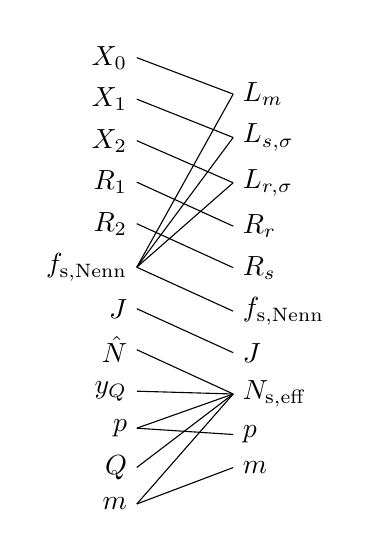
\begin{tikzpicture}[node distance=.5cm]
    % Linke Seite
    \begin{scope}[]
    	    \matrix[column 1/.style={anchor=base east}]{
             \node[] (X0) {$X_0$}; \\
             \node[] (X1) {$X_1$}; \\
             \node[] (X2) {$X_2$}; \\
             \node[] (R1) {$R_1$}; \\
             \node[] (R2) {$R_2$}; \\
             \node[] (fsNennl) {$f_{\mathrm{s,Nenn}}$};\\
             \node[] (Jl) {$J$};\\
             \node[] (N) {$\hat N$};\\
             \node[] (yQ) {$y_Q$};\\
             \node[] (pl) {$p$};\\
             \node[] (Q) {$Q$};\\
             \node[] (ml) {$m$};\\
        };
    \end{scope}
    % Rechte Seite
    \begin{scope}[xshift=2.5cm]
    	    \matrix[column 1/.style={anchor=base west}]{
             \node[] (Lm) {$L_m$}; \\
             \node[] (Lssigma) {$L_{s,\sigma}$};\\
             \node[] (Lrsigma) {$L_{r,\sigma}$};\\
             \node[] (Rr) {$R_r$};\\
             \node[] (Rs) {$R_s$};\\
             \node[] (fsNenn) {$f_{\mathrm{s,Nenn}}$};\\
             \node[] (J) {$J$};\\
             \node[] (Neff) {$N_{\mathrm{s,eff}}$};\\
             \node[] (p) {$p$};\\
             \node[] (m) {$m$};\\
        };
    \end{scope}
    \draw (Lm.west) edge (X0.east)
                    edge (fsNennl.east);

    \draw (Lssigma.west) edge (X1.east)
                    edge (fsNennl.east);

    \draw (Lrsigma.west) edge (X2.east)
                    edge (fsNennl.east);

    \draw (Neff.west) edge (N.east)
                      edge (pl.east)
                      edge (Q.east)
                      edge (ml.east)
                      edge (yQ.east);

    \draw (Rr.west) edge (R1.east);

    \draw (Rs.west) edge (R2.east);

    \draw (fsNenn.west) edge (fsNennl.east);

    \draw (p.west) edge (pl.east);

    \draw (m.west) edge (ml.east);

    \draw (J.west) edge (Jl.east);
\end{tikzpicture}

%             \node[] (XN) {$X_N$}; \\
%             \node[below=of XN] (XD) {$X_D$}; \\
%             \node[below=of XD] (XD') {$X_D'$}; \\
%             \node[below=of XD'] (XD'') {$X_D''$}; \\
%             \node[below=of XD''] (XQ) {$X_Q$}; \\
%             \node[below=of XQ] (XQ'') {$X_Q''$}; \\
%             \node[below=of XQ''] (XS) {$X_S$}; \\
%             \node[below=of XS] (fsN) {$f_{s,N}$}; \\
%             \node[below=of fsN] (Rs) {$R_s$}; \\
%             \node[below=of Rs] (TD0') {$T_{D0}'$}; \\
%             \node[below=of TD0'] (TD'') {$T_D''$}; \\
%             \node[below=of TD''] (TQ'') {$T_Q''$}; \\
	\caption{Zusammenhang zwischen den Parametern aus der Auslegung und der Simulation der Erregermaschine \label{fig:WebErr}}
\end{figure}

\section{Reglerparameter}\label{sec:Reglerparameter}

\begin{longtable}[]{@{}lll@{}}
\caption{Reglerparameter des Spannungsreglers, ausgelesen aus der Anlage}\tabularnewline
\toprule
Parameter & Dezimalwert & Hexadezimalwert\footnote{16 bit signed Integer}\tabularnewline
\midrule
\endfirsthead
\toprule
Parameter & Dezimalwert & Hexadezimalwert\tabularnewline
\midrule
\endhead
\footnotetext{16 bit signed Integer}
\texttt{Ts} & 0,00078125 & -\tabularnewline
\texttt{UgenCtrlPP\_G} & 2048 & 0x800\tabularnewline
\texttt{UgenCtrlPP\_D} & 256 & 0x100\tabularnewline
\texttt{UgenCtrlPP\_LL} & 6144 & 0x1800\tabularnewline
\texttt{UgenCtrlPP\_UL} & 8192 & 0x2000\tabularnewline
\texttt{UgenCtrlP\_D} & 256 & 0x100\tabularnewline
\texttt{UgenCtrlP\_LL} & -32768 & 0x8000\tabularnewline
\texttt{UgenCtrlP\_UL} & 32767 & 0x7FFF\tabularnewline
\texttt{UgenCtrlI\_G} & 304 & 0x130\tabularnewline
\texttt{UgenCtrlI\_D} & 4096 & 0x1000\tabularnewline
\texttt{UgenCtrlI\_LL} & 0 & 0x0\tabularnewline
\texttt{UgenCtrlI\_UL} & 32767 & 0x7FFF\tabularnewline
\texttt{UgenCtrlD\_G} & 27648 & 0x1000\tabularnewline
\texttt{UgenCtrlD\_D} & 256 & 0x5A00\tabularnewline
\texttt{UgenCtrlD\_T} & 2048 & 0x800\tabularnewline
\texttt{UgenCtrlD\_LL} & 32768 & 0x8000\tabularnewline
\texttt{UgenCtrlD\_UL} & 32767 & 0x7FFF\tabularnewline
\texttt{UgenCtrlLL} & 0 & 0x0\tabularnewline
\texttt{UgenCtrlUL} & 14336 & 0x2000\tabularnewline
\bottomrule
\end{longtable}

\begin{longtable}[]{@{}ll@{}}
\caption{Parameter für die Spannungsumwandlung, die Reglersteuerung und den Sollspannungsgeber}\label{tab:OffsetMap}\tabularnewline
\toprule
Parameter & Wert\tabularnewline
\midrule
\endfirsthead
\caption{Parameter für die Spannungsumwandlung, die Reglersteuerung und den Sollspannungsgeber}\tabularnewline
\toprule
Parameter & Wert\tabularnewline
\midrule
\endhead
\texttt{offset\_Map.I1} & 0\tabularnewline
\texttt{offset\_Map.I2} & 32767\tabularnewline
\texttt{offset\_Map.O1} & 0\tabularnewline
\texttt{offset\_Map.O2} & 80\tabularnewline
\texttt{offset\_Map1.I1} & 0\tabularnewline
\texttt{offset\_Map1.I2} & 0\tabularnewline
\texttt{offset\_Map1.O1} & 0\tabularnewline
\texttt{offset\_Map1.O2} & 3888 / 256\tabularnewline
\texttt{controlOn.startTime} & 0,7\tabularnewline
\texttt{controlOn.startValue} & \texttt{false}\tabularnewline
\texttt{V\_set.duration} & 0,3\tabularnewline
\texttt{V\_set.height} & 115\tabularnewline
\texttt{V\_set.startTime} & 0,7\tabularnewline
\bottomrule
\end{longtable}

\section{Weitere}\label{weitere}

\begin{longtable}[]{@{}ll@{}}
\caption{Allgemeine Parameter, Parameter für die Netzspeisung und
Parameter für die Last}\tabularnewline
\toprule
\begin{minipage}[b]{0.31\columnwidth}\raggedright
Parameter\strut
\end{minipage} & \begin{minipage}[b]{0.63\columnwidth}\raggedright
Wert\strut
\end{minipage}\tabularnewline
\midrule
\endfirsthead
\toprule
\begin{minipage}[b]{0.31\columnwidth}\raggedright
Parameter\strut
\end{minipage} & \begin{minipage}[b]{0.63\columnwidth}\raggedright
Wert\strut
\end{minipage}\tabularnewline
\midrule
\endhead
\begin{minipage}[t]{0.31\columnwidth}\raggedright
\texttt{simData.JRotor}\strut
\end{minipage} & \begin{minipage}[t]{0.63\columnwidth}\raggedright
1,58\strut
\end{minipage}\tabularnewline
\begin{minipage}[t]{0.31\columnwidth}\raggedright
\texttt{simData.VNominal}\strut
\end{minipage} & \begin{minipage}[t]{0.63\columnwidth}\raggedright
410\strut
\end{minipage}\tabularnewline
\begin{minipage}[t]{0.31\columnwidth}\raggedright
\texttt{simData.fNominal}\strut
\end{minipage} & \begin{minipage}[t]{0.63\columnwidth}\raggedright
50\strut
\end{minipage}\tabularnewline
\begin{minipage}[t]{0.31\columnwidth}\raggedright
\texttt{ramp\_net.height}\strut
\end{minipage} & \begin{minipage}[t]{0.63\columnwidth}\raggedright
\texttt{simData.VNominal\ *\ sqrt(2)}\strut
\end{minipage}\tabularnewline
\begin{minipage}[t]{0.31\columnwidth}\raggedright
\texttt{ramp\_net.duration}\strut
\end{minipage} & \begin{minipage}[t]{0.63\columnwidth}\raggedright
0,5\strut
\end{minipage}\tabularnewline
\begin{minipage}[t]{0.31\columnwidth}\raggedright
\texttt{fan.J}\strut
\end{minipage} & \begin{minipage}[t]{0.63\columnwidth}\raggedright
\texttt{simData.JRotor}\strut
\end{minipage}\tabularnewline
\begin{minipage}[t]{0.31\columnwidth}\raggedright
\texttt{fan.a}\strut
\end{minipage} & \begin{minipage}[t]{0.63\columnwidth}\raggedright
\texttt{(fixed\ =\ false)}\strut
\end{minipage}\tabularnewline
\begin{minipage}[t]{0.31\columnwidth}\raggedright
\texttt{fan.phi}\strut
\end{minipage} & \begin{minipage}[t]{0.63\columnwidth}\raggedright
\texttt{(displayUnit\ =\ "rad")}\strut
\end{minipage}\tabularnewline
\begin{minipage}[t]{0.31\columnwidth}\raggedright
\texttt{fan.w}\strut
\end{minipage} & \begin{minipage}[t]{0.63\columnwidth}\raggedright
\texttt{(fixed\ =\ true,\ start\ =\ 314)}\strut
\end{minipage}\tabularnewline
\begin{minipage}[t]{0.31\columnwidth}\raggedright
\texttt{frequency.k}\strut
\end{minipage} & \begin{minipage}[t]{0.63\columnwidth}\raggedright
8 / (2 * pi)\strut
\end{minipage}\tabularnewline
\begin{minipage}[t]{0.31\columnwidth}\raggedright
\texttt{loadTimeTable.extra­po­lation}\strut
\end{minipage} & \begin{minipage}[t]{0.63\columnwidth}\raggedright
\texttt{Modelica.­Blocks.­Types.­Extra­po­lation.­HoldLastPoint}\strut
\end{minipage}\tabularnewline
\begin{minipage}[t]{0.31\columnwidth}\raggedright
\texttt{loadTimeTable.fileName}\strut
\end{minipage} & \begin{minipage}[t]{0.63\columnwidth}\raggedright
``Laststufen\_timetable.txt''\strut
\end{minipage}\tabularnewline
\begin{minipage}[t]{0.31\columnwidth}\raggedright
\texttt{loadTimeTable.smooth­ness}\strut
\end{minipage} & \begin{minipage}[t]{0.63\columnwidth}\raggedright
\texttt{Modelica.­Blocks.­Types.­Smooth­ness.­ConstantSegments}\strut
\end{minipage}\tabularnewline
\begin{minipage}[t]{0.31\columnwidth}\raggedright
\texttt{loadTimeTable.table}\strut
\end{minipage} & \begin{minipage}[t]{0.63\columnwidth}\raggedright
{[}0, 0.705328, 0.00021048; 6.2, 0.352664, 0.00010524{]}\strut
\end{minipage}\tabularnewline
\begin{minipage}[t]{0.31\columnwidth}\raggedright
\texttt{loadTimeTable.tableName}\strut
\end{minipage} & \begin{minipage}[t]{0.63\columnwidth}\raggedright
``laststufen''\strut
\end{minipage}\tabularnewline
\begin{minipage}[t]{0.31\columnwidth}\raggedright
\texttt{loadTimeTable.table­OnFile}\strut
\end{minipage} & \begin{minipage}[t]{0.63\columnwidth}\raggedright
\texttt{false}\strut
\end{minipage}\tabularnewline
\bottomrule
\end{longtable}
